\documentclass[times, doublespace]{anzsauth}
\usepackage{moreverb}
\usepackage{url}
\usepackage{grffile}
\usepackage{lineno}
% \usepackage{lmodern}
\usepackage{lipsum}
\usepackage[UKenglish]{isodate}

\usepackage[acronym]{glossaries}
\newacronym[shortplural={ATIS}]{atis}{ATIS}{advanced traveller information system}
\newacronym{avl}{AVL}{automatic vehicle location}
\newacronym{apc}{APC}{automatic passenger counter}
\newacronym{rti}{RTI}{real-time information}
\newacronym{gps}{GPS}{Global Positioning System}
\newacronym{api}{API}{application programming interface}
\newacronym{gtfs}{GTFS}{general transit feed specification}
\newacronym{knn}{KNN}{$k$-nearest neighbour}
\newacronym{ann}{ANN}{artificial neural networks}
\newacronym{svm}{SVM}{support vector machines}
\newacronym{kf}{KF}{Kalman filter}
\newacronym{ekf}{EKF}{extended Kalman filter}
\newacronym{pf}{PF}{particle filter}
\newacronym{mcmc}{MCMC}{Markov chain Monte Carlo}
\newacronym[longplural={expected times of arrival}]{eta}{ETA}{expected time of arrival}
\newacronym{at}{AT}{Auckland Transport}
\newacronym{pt}{PT}{public transport}
\newacronym{ui}{UI}{user interface}
\newacronym{osm}{OSM}{OpenStreetMap}

\newcommand{\bv}{\boldsymbol{v}}
\newcommand{\bz}{\boldsymbol{z}}
\newcommand{\bw}{\boldsymbol{w}}
\newcommand{\bR}{\boldsymbol{R}}
\newcommand{\btheta}{\boldsymbol{\theta}}

\def\volumeyear{2018}
\linenumbers

\begin{document}
\cleanlookdateon
\runningheads{Short title of paper}{TOM~ELLIOTT AND THOMAS~LUMLEY}
\title{Long name of the paper}
\author{Tom Elliott\corrauth~and~Thomas~Lumley}
\affiliation{University of Auckland}
\address{
    Department of Statistics, University of Auckland, 
    Auckland 1142, New Zealand\\
    Email: \texttt{tom.elliott@auckland.ac.nz}
}

\begin{abstract}
Predicting transit vehicle arrival time is a somewhat complex procress.
Road networks are dynamic, and can change from free-flowing to highly congested
very quickly.
Any reliable prediction framework needs to be able to respond to these changes,
but also to future trends, such as typical changes to traffic flow
at peak times, based on hisorical data.
Of course, the major constraint on any prediction framework is going to be
computational efficiency.
Due to the realtime nature of the problem, predictions need to be 
available as soon as possible after observing the vehicles' positions,
which are updated approximately every 30~seconds.
In this paper, we describe our C++ implementation of a particle filter to estimate
vehicle state in combination with a network state model,
allowing us to model transit vehicle flow through the network.
While our application here is being testing in Auckland, New Zealand,
we hope that our methods are general enough to be applied to any
transit network that uses GTFS.
Preliminary results show that, with suitable hardware,
the framework is fast enough while retaining the complexity necessary
to incorporate as much information as necessary to predict arrival times.
\end{abstract}

\keywords{particle filter; Kalman filter; transit modeling;
          transit networks; statistical computing; applications; gtfs}

\maketitle
\section{Introduction}
\label{sec:intro}


In public transport, \rt information (RTI)---%
most notably estimated times of arrival (ETAs)---%
keeps transport users informed of changes to their commute,
and plan their journey accordingly.
Previous research has shown that perceived waiting time is less
when arrival time information is available \citep{TCRP_2003b},
but here in Auckland, RTI is highly unreliable,
resulting in frustration and deterence of public transport users.
Inaccurate ETAs are a major source of this frustration,
as they fluctuate---sometimes dramatically---over time.
The cause of this can be complex, such as unexpected traffic congestion,
or simply because of poor schedule calibration.
Furthermore, buses are shown as \emph{on-time} 
if they are not present in the \rt system and have not been manually cancelled,
in which case ETAs are based solely on scheduled arrival times.
Once the scheduled arrival time has passed,
the service is removed from the \rt board,
leaving passengers unsure as to when---if at all---their bus will show up,
a phenomenon referred to as ``ghost buses'' by transport bloggers.


Arrival time prediction is only as reliable as the underlying model,
and while a lot of work has gone into developing public transport vehicle models
\citep{Cathey_2003,Jeong_2005,Yu_2011,Hans_2015},
many public transport providers---notably Auckland Transport---useno formal model is used.
Instead, ETAs are based solely on the scheduled arrival time
adjusted by the vehicle's arrival or departure delay at the most recent stop, 
\emph{if available},
the primary assumption being that the schedule is valid,
and secondly that there is no unusual congestion along the route;
neither of these are valid,
particularly in our test area of Auckland, New Zealand,
where infrastructure for buses (such as priority lanes) is limited,
and bus drivers, in general, 
do not actively adhere to the schedule.


A more robust modelling and prediction framework 
based on \rt congestion information would avoid making these assumptions.
Such a framework should consist of a robust vehicle model to estimate the position and speed
of transit vehicles from \rt GPS data,
and secondly a means of combining speed information from vehicles
to model traffic flows,
which can then be used to improve arrival time predictions.
Several vehicle modelling approaches were explored, 
including the Kalman filter \citep{Dailey_2001,Cathey_2003},
machine learning models \citep{Yu_2006,Chang_2010},
and the particle filter \citep{Hans_2015}.


The particle filter has proven itself as a robust option for
\rt vehicle tracking applications
\citep{Gustafsson_2002,Davidson_2011},
and as computational power has increased over recent years,
a strong competitor for \rt applications.
\cite{Ulmke_2006} showed it to handle situations where traditional
(i.e., Kalman filter) methods break down:
the particle filter retained the accurate uncertainty about the location
where there was a lack of information,
an important property for our model in which we expect
many situations where there are sparse observations
and a strongly multimodal distribution.
By using a particle filter,
we were able to develop a simple, flexible framework
which is robust to the type of data we expect to observe.


The second component involves estimating traffic conditions throughout the transport network
using the information obtained from the vehicle model.
\cite{Yu_2010} improved prediction accuracy by using the travel times
of buses travelling along the same route.
A similar method presented by \cite{Hans_2015}
used headway, the time between consecutive vehicles at a point on the route,
as a predictor of travel time.
Since these approaches only work well on high frequency routes,
\cite{Yu_2011} showed further improvements by combining travel times 
from several routes;
however, this was limited to predefined converging routes.
In general, however, no comprehensive network modelling approach has been proposed using
solely GPS position data to model and account for congestion when estimating arrival times.


In Section~\ref{sec:models} of this paper, 
we describe the \rt vehicle and network state models
used to estimate traffic congestion using the transit vehicles
travelling through the network in real-time,
and in Section~\ref{sec:rt} we demonstrate the feasibility of using a particle filter
in \rt to model transit vehicles,
and evaluate its performance.
First, however, we descibe how we construct a
transit road network from GTFS data in Section~\ref{sec:gtfs}.




\section{Working with \rt transit data}
\label{sec:gtfs}

GTFS (general transit feed specification)
is an API (application programming interface) specification for transit data
detailing how it should be organised,
making access easier for application developers.
Developed and maintained by Google \citep{GoogleDevelopers_2006},
who use it in Google Maps Transit Directions,
it is used by over 1100~transit providers around the world\footnote{%
source: \url{http://transitfeeds.com} as of August 2019},
including here in Auckland, New Zealand.
An advantage of this standardised format is that,
provided an application depends solely on GTFS data,
after developing it locally in Auckland it can be deployed to any other GTFS-based
public transport system with minimal modification.


There are two components to GTFS.
The first, \emph{GTFS static}, includes information about
\begin{itemize}
\item \emph{stops}, a physical location where passengers can embark and disembark the vehicle;
\item \emph{routes}, a sequence of two or more stops displayed as a single service;
\item \emph{trips}, an instance of a route occurring at a specific time of day;
\item \emph{schedules}, specifying the arrival (and departure) times for each bus at each of its stops; 
\item and \emph{shapes}, the sequence of points defining a vehicle's path along a route.
\end{itemize}
The second component is \emph{GTFS-realtime},
which is only available in a subset of the providers due to the requirement of 
on board GPS tracking devices and a central server.
It provides a standardised format for sharing vehicle positions and trip delays,
and are typically accessed by developers via an API that can be used in \rt applications.

As mentioned in Section~\ref{sec:intro},
there are some major issues with the arrival time prediction method currently
deployed in Auckland,
which is based entirely on \emph{GTFS-realtime} trip updates---%
vehicle positions are used only to display \emph{where} the bus is.
Trip updates are reported whenever a vehicle arrives at or departs from a stop,
and includes the delay between the scheduled and actual arrival times,
which is propagated to all future stops to update their ETAs.
As already mentioned, this assumes that the schedule is well calibrated,
and that the time between stops
is representative of the real-world travel time between them. 
Figure~\ref{fig:gtfs-delays} demonstrates the fallibility of the current approach,
where we see the progressive lateness causing the passenger's ETA to 
jump each time the bus arrives at a stop.
An estimation approach using \rt travel times 
between stops would seem more adequate.

\begin{figure}[tb]
    \centering
    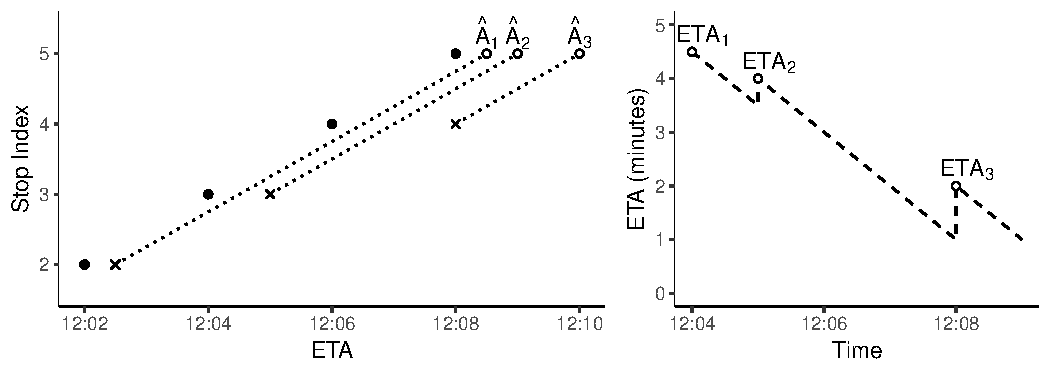
\includegraphics[width=0.9\textwidth]{figures/02_gtfs_delays.pdf}
    \caption{
        On the left, scheduled arrival times are shown as solid points,
        for several stops along a route. The actual arrival times
        are shown with crosses,
        and the GTFS-based ETAs for stop 5, $\hat A_1$, $\hat A_2$, and $\hat A_3$, are also shown.
        On the right,
        for a passenger arriving at stop 5 at 12:04,
        the ETA over time is shown, demonstrating the fluctuation in
        arrival time as the bus arrives at each stop.
    }
    \label{fig:gtfs-delays}
\end{figure}



\subsection{Transit network construction}
\label{sec:network_build}

The primary predictor of arrival time is 
the travel time along roads between where the bus is \emph{now},
and the stop at which a passenger is waiting.
In most applications, however, this vital information is unavailable, at least directly.
In order to compute travel times efficiently
and make use of all available data pooled across multiple routes,
we constructed a \emph{road network},
allowing us to model roads directly,
such that every bus travelling along a road contributes to its state,
which can in turn be used to predice travel times for all upcoming buses 
travelling along the road,
irrespective of the route they are servicing.


To construct the transit network,
routes were split into spatially identifiable segments,
each representative of a physical road,
using bus stops as nodes in the network
and the connecting roads as edges
(Figure~\ref{fig:network_creation}).
In this way, routes that service the same subsequence of stops
all contribute to traffic flow information for the connecting roads.
Although there are several drawbacks to this method,
such as road segment overlaps where routes merge between stops,
our approach is sufficient for the purposes of assessing the \rt 
faesibilty of our proposed prediction framework.



\begin{figure}[tb]
    \centering
    \begin{subfigure}{0.7\textwidth}
        \centering
        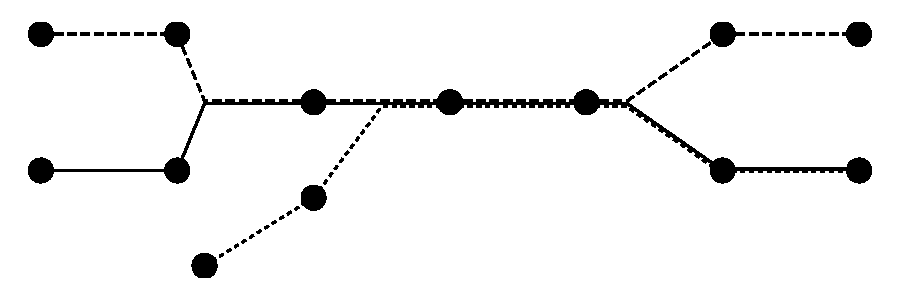
\includegraphics[width=0.95\textwidth]{figures/02_network_segments_1.pdf}
        \caption{Raw GTFS route shapes}
        \label{fig:network_creation_1}
    \end{subfigure} \\
    \begin{subfigure}{0.7\textwidth}
        \centering
        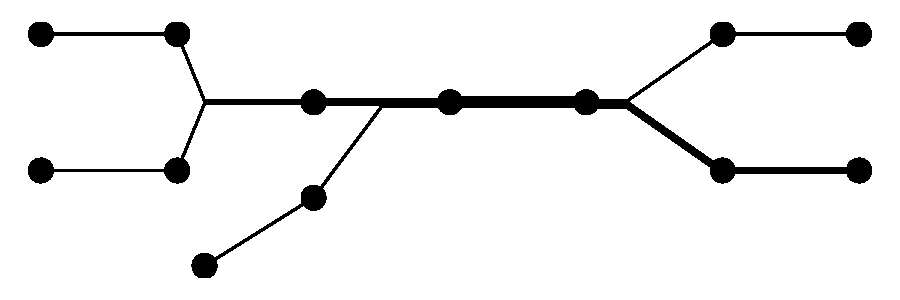
\includegraphics[width=0.95\textwidth]{figures/02_network_segments_2.pdf}
        \caption{GTFS-based road network}
        \label{fig:network_creation_2}
    \end{subfigure}
    \caption{
        Bus stops (shown as dots above) can be serviced by more than one route, 
        as shown in (a), with different line types representing three separate routes.
        The constructed road network, using stops as nodes, is shown in (b),
        in which the connecting lines represent physical road segments,
        with line width proportional to the number of individual routes 
        travelling along that road.
    }
    \label{fig:network_creation}
\end{figure}


\subsection{Real-time vehicle locations}
\label{sec:realtime_data}

\emph{GTFS-realtime} provides the positions of vehicles in a transit network.
The data consists of the time $t_k$ that the position was last updated,
the GPS position of the vehicle, $\bY_k$, 
and information about the trip being serviced.
In Auckland, vehicle positions are updated with a frequency of anywhere between 10~seconds and several minutes,
so there is often a lot of uncertainty about a vehicle's intermediate trajectory,
particularly when there are one or more bus stops along the way.
It is also possible for a bus to remain stationary,
for example due to heavy congestion,
so the number of possible trajectories rapidly increases with 
the time between observations.


One important consideration regarding Auckland Transport's \rt implementation is that
buses are programmed to report their location when arriving at or departing from
bus stops, as well as some major intersections.
To further complicate this,
these positions can be preemptive,
for example when approaching a queue of traffic at an intersection,
the way-point may be triggered before the bus physically gets there,
so consecutive observations may show what appears to be a bus travelling backwards.
To handle this, we compute the approximate distance travelled, $\tilde x_k$,
of the vehicle by finding the nearest point on the path to the observation;
if this has decreased, the current state (based on the preemtive observation)
is rejected and the vehicle reverted
to its previous state before continuing.
So at the cost of losing one (likely invalid) observation,
we are able to improve particle filter performance
when this situation is encountered.


\section{The Models}
\label{sec:models}

Real-time tracking applications often use
a Bayesian filtering approach,
or recursive Bayesian estimation,
in which the data is processed sequentially instead of all at once,
reducing computational demands
\citep{Anderson_2012}.
These models assume an underlying Markov process with state $\boldsymbol{\mathcal{X}}_k$,
an $n\times1$ column vector,
with system noise $\boldsymbol{\omega}_k\sim\mathrm{N}(\boldsymbol{0},\mathcal{Q})$ 
of which observations $\boldsymbol{\mathcal{Y}}_k$,
an $m\times1$ column vector, are made
with error $\boldsymbol{\nu}_k\sim\mathrm{N}(\boldsymbol{0},\mathcal{R})$,
giving the following general model:
\begin{equation}
\label{eq:rbe_model}
\begin{split}
\boldsymbol{\mathcal{X}}_k &= f(\boldsymbol{\mathcal{X}}_{k-1}, \boldsymbol{\omega}_k) \\
\boldsymbol{\mathcal{Y}}_k &= h(\boldsymbol{\mathcal{X}}_k) + \boldsymbol{\nu}_k
\end{split}
\end{equation}
The transition function $f:\mathbb{R}^n\mapsto\mathbb{R}^n$ 
describes the relationship between consecutive states,
while the measurement function $h:\mathbb{R}^n\mapsto\mathbb{R}^m$ is a deterministic function
mapping the underlying state to the observable state,
of which noisy measurements are made.



The following sections describe the two models used in this application,
both of which are examples of a Bayesian filter.
The first, implemented using a particle filter, estimates vehicle states
with the primary goal of estimating road travel times from a sequence of GPS positions;
the second uses these travel times to update road states 
and is implemented using an \emph{information filter},
a variant of the Kalman filter \citep{Anderson_2012}.



\subsection{Real-time vehicle model}
\label{sec:pf}

The underlying vehicle state at time $t_k$ consists of
the vehicle's distance travelled $x$ in meters along the route and
its speed $\dot x$ in meters per second.
These are combined into the state vector
$\bX_k = \left[x_k\ \dot x_k\right]^\top$,
of which observations $\bY_k$ are made using a GPS
with error $\omega^2$,
giving the longitude $\lambda_k$ and latitude $\phi_k$ of the vehicle
as $\bY_k = \left[\lambda_k\ \phi_k \right]^\top$.
We use a particle filter to estimate $\bX_k$,
due to its flexibility and proven robustness
in recent vehicle modelling applications \citep{Ulmke_2006,Hans_2015}.
In addition, it makes it trivial to estimate travel times
$\bz = (z_1,\ldots,z_L)^\top$, in seconds, along road segments
as the vehicle traverses the route.


The primary advantage of the particle filter is its handling of multimodality,
as demonstrated in Figure~\ref{fig:pf_state_predict},
which is a common feature of the proposal distribution, particularly around bus stops.
Another advantage is that the likelihood function is intuitively based
on the physical distance between the vehicle observation and the state's
estimate of the true location, $h(\bX_k)$ (Section~\ref{sec:pf_update}).
Conversely, particle filter methods are computationally demanding,
requiring an increasing number of particles as model complexity and
number of parameters increases \citep{Carpenter_1999}.
Section~\ref{sec:rt} describes our implementation of the particle filter
and its \rt performance.

\begin{figure}[p]
    \centering
    \begin{subfigure}[t]{1\textwidth}
        \centering
        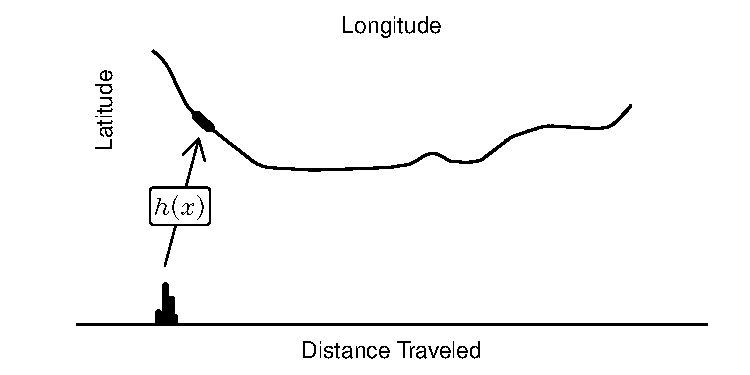
\includegraphics[width=0.7\textwidth]{figures/03_particle_filter_1.pdf}
        \caption{
            Vehicle state is mapped to observation space by the
            measurement function $h$.   
        }
        \label{fig:pf_state_prev}
    \end{subfigure}\\
    \begin{subfigure}[t]{0.9\textwidth}
        \centering
        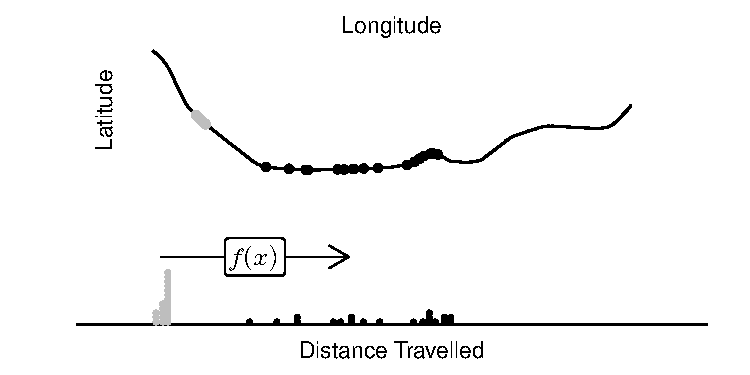
\includegraphics[width=0.7\textwidth]{figures/03_particle_filter_2.pdf}
        \caption{
            The transition function $f$ predicts the future state 
            of each particle.
        }
        \label{fig:pf_state_predict}
    \end{subfigure}\\
    \begin{subfigure}[t]{0.9\textwidth}
        \centering
        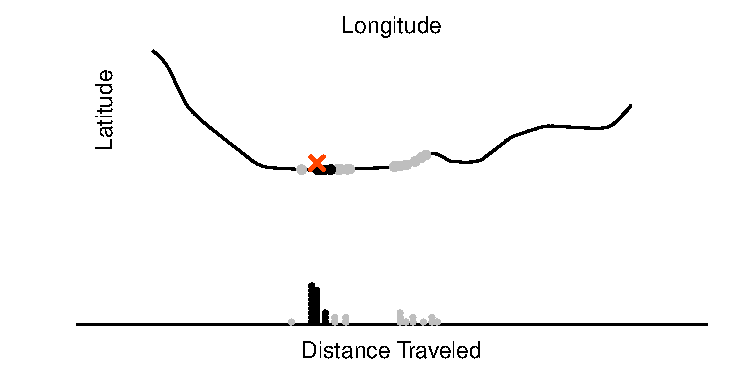
\includegraphics[width=0.7\textwidth]{figures/03_particle_filter_4.pdf}
        \caption{
            The state is updated by weighted resampling based on distance
            of particle to observation.
        }
        \label{fig:pf_state_predict2}
    \end{subfigure}
    \caption{
        The particle filter approximates vehicle state using a set of 
        discrete points (a), which are each mutated independently (b)
        to predict the next state.
        The measurement function $h$ allows each particle state
        to be mapped to a GPS coordinate (a),
        which can be compared to the observed location (c)
        to calculate each particle's likelihood to compute resampling weights.
    }
    \label{fig:pf_state}
\end{figure}

\afterpage{\clearpage}

In a particle filter, the posterior distribution of the state at time $t_{k-1}$
is represented by a set of discrete points, or particles, (Figure~\ref{fig:pf_state_prev}),
each with an associated weight $W_{k-1}^{(i)}$.
The state is expressed using the Dirac delta function $\dot\delta(\cdot)$,
so that
\begin{equation*}
p(\bX_{k-1} | \bY_{1:k-1}) \approx 
    \sum_{i=1}^N W_{k-1}^{(i)} \dot\delta(\bX_{k-1} - \bX_{k-1}^{(i)})
\end{equation*}
each of which is independently updated or \emph{mutated} using the transition function $f$ (Figure~\ref{fig:pf_state_predict}),
\begin{equation*}
p(\bX_k | \bX_{k-1}) \approx 
    \sum_{i=1}^N W_{k-1}^{(i)} \dot\delta(\bX_{k} - f(\bX_{k-1}^{(i)}, \boldsymbol{\psi})),
\end{equation*}
where $\boldsymbol{\psi}$ is a vector containing all of the necessary model parameters
(Section~\ref{sec:pf_prediction}).
After mutation, 
the state is updated by reweighting the particles using the likelihood $p(\bY_k | \bX_k^{(i)})$ 
(Section~\ref{sec:pf_update}) and standardising so $\sum_{i=1}^N W_k^{(i)} = 1$,
\begin{equation*}
W_k^{(i)} = \frac{W_{k-1}^{(i)} p(\bY_k | \bX_k^{(i)})}{
    \sum_{j=1}^N W_{k-1}^{(j)} p(\bY_k | \bX_k^{(j)})
}
\end{equation*}
which gives us the final posterior state estimate
\begin{equation*}
p(\bX_k | \bY_k) \approx  
    \sum_{i=1}^N W_{k}^{(i)} \dot\delta(\bX_{k} - \bX_{k}^{(i)}).
\end{equation*}

One problem with particle filters is degeneration,
which occurs when the particle sample no longer approximates the target distribution
due to the particles becoming too diverse
and all of the weight falls onto only a small number of them.
This occurs naturally over time, but the rate at which it occurs depends 
on a relationship between how well the transition function predicts future states,
and the variance of those predictions (system noise).
To avoid degeneration,
particle filters use \emph{importance resampling}
using importance weights $\{W_k^{(1)}, \ldots, W_k^{(N)}\}$,
thereby removing improbable particles and replacing them with more probable ones,
as demonstrated in Figure~\ref{fig:pf_state_predict2}.
However, resampling requires sorting $N$ particles,
which is of $\mathcal{O}(N\log N)$ complexity,
so to reduce computational costs, resampling is performed only when
the effective sample size $N_{\text{eff}} = 1 / \sum_i (W_k^{(i)})^2$
falls below a specified threshold $N_{\text{thres}}$
\citep{Gustafsson_2002}.
We used a fixed threshold value of $N_{\text{thres}} = N/4$
for the current work.


\subsubsection{Vehicle transition function}
\label{sec:pf_prediction}

The particle filter allows us to flexibly model bus behaviour,
which currently includes
\begin{enumerate}
\item non-constant speed along roads (between observations), and
\item bus stop behaviour, which involves optional stopping and waiting times
    while passengers board and disembark.
\end{enumerate}
The transition function consists of two models,
one for each of the above behaviours.
The first models the speed and distance travelled by the vehicle 
by using Newton's Laws of Motion,
which, letting $\delta_k = t_k - t_{k-1}$, is
\begin{equation}
\label{eq:trans_newton}
\bX_k^{(i)} = f(\bX_{k-1}^{(i)}, \delta_k, \epsilon_k^{(i)}) = 
    \begin{bmatrix}
        x_{k-1}^{(i)} + \delta_k(\dot x_{k-1}^{(i)} + \epsilon_k^{(i)}) \\
        \dot x_{k-1}^{(i)} + \epsilon_k^{(i)}
    \end{bmatrix},
\end{equation}
where $\epsilon_k^{(i)}\sim\mathrm{N}_T(0, \sigma^2)$, truncated to the interval
$(-\dot x_{k-1}^{(i)}, 30 - \dot x_{k-1}^{(i)})$,
which ensures vehicle speed is always positive and less than 30~m/s
(approximately 110~km/h).


The second vehicle behaviour requires a model of bus stop wait times.
When the vehicle is approaching stop $j$,
it stops with some probability $\pi_j$.
If it does not stop, the remaining travel time $\delta_k$ is unaltered;
otherwise, the bus waits for a minimum of $\gamma$ seconds---this 
accounts for deceleration, opening and closing of doors, and acceleration
\citep{Hans_2015}---and then waits while passengers board and disembark,
which is assumed to be exponentially distributed with mean $\tau_j$.
This leads to the following model,
\begin{equation}
\label{eq:trans_stop}
\begin{split}
p_j^{(i)} &\sim \mathrm{Bernoulli}(\pi_j) \\
\tilde d_j^{(i)} &\sim \mathrm{Exponential}(\tau_j) \\
d_j^{(i)} &= p_j^{(i)}(\gamma + \tilde d_j^{(i)}).
\end{split}
\end{equation}


The model components are implemented as an algorithm,
in which (\ref{eq:trans_newton}) is evaluated iteratively one second at a time,
decreasing $\delta_k^{(i)}$ by one each time,
after initializing $\delta_k^{(i)} = \delta_k$.
In order to obtain the desired non-constant speed between observations,
$\epsilon_k^{(i)}$ is re-sampled each second,
allowing the particle's speed to vary.
This iterative approach allows the particle to approach the next stop,
at which point (\ref{eq:trans_stop}) is evaluated for the particle
and the dwell time subtracted from $\delta_k^{(i)}$.
This process continues until $\delta_k^{(i)}$ reaches zero.
The algorithm also keeps track of each particle's travel time $z_\ell^{(i)}$
along each segment $\ell$ of the route,
storing the times so that the posterior distribution of the travel time
can be computed once all particles have completed segment $\ell$:
\begin{equation}
\label{eq:post_tt}
p(z_\ell | \bY_{1:k}) \approx
    \sum_{i=1}^N W_k^{(i)} \dot\delta(z_\ell - z_\ell^{(i)}).
\end{equation}



\subsubsection{Updating state using the observation likelihood}
\label{sec:pf_update}

To compute the likelihood of the observation given each particle state,
$p(\bY_k|\bX_k^{(i)})$,
the measurement function $h$ is needed along with 
a \emph{geographical projection} function $g$ to allow comparison of $\bY_k$,
a GPS observation, with $\bX_k$, a distance travelled along the route in meters.

The measurement function $h$ computes GPS coordinates by using the 
shape information provided by GTFS and travelling $x_k$ meters along 
this two-dimensional line.
Meanwhile, we use the \emph{Equirectangular projection} \citep{Snyder_1998},
$\br = g(\bY_1 | \bY_0)$,
such that the magnitude of $\boldsymbol{r}$ is equal to the physical distance
between $\bY_0$ and $\bY_1$ and both dimensions are in meters.
Let $\bY_i = [\lambda_i, \psi_i]^\top$,
with $\lambda_i$ and $\psi_i$ measured in radians,  
and $R$ is the Earth's radius, in meters, then
\begin{equation}
\br = 
g(\bY_1 | \bY_0) = 
    \begin{bmatrix}
        r_1 \\ r_2
    \end{bmatrix} =
    R \begin{bmatrix}
        (\lambda_1 - \lambda_0)\cos\phi_0 \\
        \phi_1 - \phi_0
    \end{bmatrix}
\end{equation}
and, more importantly, the geographical distance $\mathcal{D}$ between the two 
GPS coordinates is given by
\begin{equation}
\label{eq:dist}
\mathcal{D}(\bY_0, \bY_1) = ||g(\bY_0 | \bY_1)|| = \sqrt{r_1^2 + r_2^2}.
\end{equation}


Now we assume GPS observations have a known error of $\omega^2$ meters,
and that \mbox{$\br \sim \mathrm{N}(\boldsymbol{0}, \omega^2\mathbf{I})$},
which allows us to express $\br$ in terms of two independent
standard normal random variables $z_1, z_2 \sim \mathrm{N}(0,1)$.
Now the distance between a vehicle observation $\bY_k$
and a state $\bX_k$, using (\ref{eq:dist}) and the measurement function $h$,
is expressed as
\begin{equation}
\label{eq:obs_dist}
\mathcal{D}(\bY_k, h(\bX_k)) = \sqrt{r_{k1}^2 + r_{k2}^2} 
    = \sqrt{(\omega z_1)^2 + (\omega z_2)^2}
    = \sqrt{\omega^2 (z_1^2 + z_2^2)}.
\end{equation}

Finally, it is known that the distribution of the sum of two indendent 
standard normal variables is exponentially distributed with rate $\frac{1}{2}$,
and that if $Z \sim \mathrm{Exponential}(\theta)$ then
$cZ \sim \mathrm{Exponential}(\frac{\theta}{c})$,
so the \emph{squared} distance from (\ref{eq:obs_dist}) is distributed as
\begin{equation}
\label{eq:obs_exp}
\mathcal{D}(\bY_k, h(\bX_k))^2 =
\omega^2(z_1^2 + z_2^2) \sim \mathrm{Exponential}\left(\frac{1}{2\omega^2}\right).
\end{equation}

The likelihood of the observation $\bY_k$ given a state estimate $\bX_k^{(i)}$
can now be expressed using (\ref{eq:obs_exp}) 
and the probability density function of the exponential distribution,
\begin{equation}
\label{eq:lhood}
p(\bY_k | \bX_k^{(i)}, \omega) =
\frac{1}{2\omega^2}\exp\left\{
    -\frac{\mathcal{D}(\bY_k, h(\bX_k^{(i)}))^2}{2\omega^2}
\right\},
\end{equation}
where the distance between two GPS coordinates is easily computed,
allowing for fast evaluation of (\ref{eq:lhood}) within the particle filter algorithm.


It is worth noting that this representation of the likelihood is only
possible due to the discrete nature of the particle filter state estimate;
in the Kalman filter, which has often been used in transit vehicle tracking,
the measurement \emph{matrix} is used, and requires a linear
transformation between the state and its observations.
To enable this, applications first estimate the \emph{observed distance travelled}
by snapping the GPS observations to the route,
which introduces unnecessary error and uncertainty into the model.
Our approach avoids this, which makes it more stable in locations where two 
parts of the route are close to each other,
such as at loops, where a single GPS observation might have two likely ``snapping'' points.


\subsection{Network model}
\label{sec:kf}

The primary objective of the network model is to estimate the \rt traffic conditions
(travel time) along roads in the transit network, 
and make short-term forecasts for estimating arrival times.
In this paper, we model each road segment independently,
as excluding correlations simplifies the model to not only a one-dimensional Kalman filter,
but it also means computations can be run in parallel,
greatly increasing the real-time performance of the model.


The network state $\boldsymbol\theta_c = \{\theta_c^\ell\}_{\ell = 1}^L$ is the travel time 
of transit vehicles along road segment $\ell$ at time $t_c$,
of which observations $Z_{c\ell}^{m}$
are obtained from the particle filter for vehicle $m$ at time $t_c$,
as defined in (\ref{eq:post_tt}), such that 
(after adding the $m$ superscript to identify unique vehicles), 
\begin{equation}
\label{eq:tt_obs_mean}
Z_{c\ell}^{m} = \mathrm{E}(z_{\ell}^{m} | \bY^m_{1:c}) = 
\sum_{i=1}^N (W_c^{(i)})^m (z_\ell^{(i)})^{m}.
\end{equation}
The measurement error is also estimated from the particle filter,
\begin{equation}
\label{eq:tt_obs_err}
R_{c\ell}^m = \mathrm{Var}(z_{\ell}^{m} | \bY^m_{1:c}) = 
\sum_{i=1}^N (W_c^{(i)})^m \left((z_\ell^{(i)})^{m} - Z_{c\ell}^{m}\right)^2.
\end{equation}

The model of travel times becomes a simple reduction of (\ref{eq:rbe_model}) 
to the one dimensional case, 
with $f$ and $h$ both unity,
system noise $v_{c\ell} \sim \mathrm{N}(0, \nu_\ell^2)$,
where $\nu_\ell^2$ is the average change in travel time per second
along road segment $\ell$,
the observation error $e_{c\ell}^{m} \sim \mathrm{N}(0, R_{c\ell}^{m})$,
and $\Delta_c = t_c - t_{c-1}$
\begin{equation*}
\begin{split}
\theta_c^\ell &= \theta_{c-1}^\ell + \Delta_{c\ell} v_{c\ell} \\
Z_{c\ell}^{m} &= \theta_c^\ell + e_{c\ell}^{m}
\end{split}
\end{equation*}


Since multiple vehicles can travel along a road simultaneously,
we used an information filter to implement the network model.
The information filter is a transformation of the Kalman filter in which the
\emph{information matrix} and \emph{information vector} are used in place of 
the covariance matrix and state vector, respectively,
allowing multiple observations to be added together to update the state
in a single iteration.


The state at time $t_{c-1}$ is parameterised by its mean and variance,
conditional on $\boldsymbol{Z}_{1:c-1,\ell}$, 
the data from all vehicles up until time $t_{c-1}$,
\begin{equation*}
\hat \theta_{c-1|c-1}^\ell = 
\mathrm{E}(\theta_{c-1}^\ell | \boldsymbol{Z}_{1:c-1,\ell})
\quad\text{and}\quad
P_{c-1|c-1}^\ell = 
\mathrm{Var}(\theta_{c-1}^\ell | \boldsymbol{Z}_{1:c-1,\ell})
\end{equation*}
respectively,
which are predicted from the previous state estimate using the predictive model
\begin{align*}
\label{eq:kf_transition}
\hat \theta^\ell_{c|c-1} &= \hat \theta^\ell_{c-1|c-1} \\
P^\ell_{c|c-1} &= P^\ell_{c-1|c-1} + (\Delta_{c\ell} \nu_{c\ell})^2
\end{align*}

For the update step, the parameters are transformed into an information
space parameterised by the information matrix $U^\ell_c = (P_{c|c-1}^\ell)^{-1}$
and the information vector $u^\ell_c~=~\hat \theta^\ell_{c|c-1} (P^\ell_{c|c-1})^{-1}$.
The travel time estimate of vehicle $m$ along segment $\ell$,
along with its uncertainty, 
as defined in (\ref{eq:tt_obs_mean}) and (\ref{eq:tt_obs_err}), respectively,
are transformed to a measurement information covariance matrix 
$B_{c\ell}^{m}~=~(R_{c\ell}^m)^{-2}$
and measurement information vector $b_{c\ell}^{m}~=~Z_{c\ell}^{m} (R_{c\ell}^{m})^{-2}$.
The total information is the sum of the information over all $M_{c\ell}$ vehicles
that traversed segment $\ell$ in the time interval $(t_{c-1}, t_c]$,
so the update equation is
\begin{align*}
U^\ell_{c|c} &= U^\ell_{c|c-1} + \sum_{m=1}^{M_{c\ell}} B_{c\ell}^{m} \\
\hat u^\ell_{c|c} &= \hat u^\ell_{c|c-1} + \sum_{m=1}^{M_{c\ell}} b_{c\ell}^{m}.
\end{align*}
The desired parameter estimates are obtained 
by the inverse transformations
\begin{equation*}
\hat \theta^\ell_{c|c} = \frac{\hat u^\ell_{c|c}}{U^\ell_{c|c}} 
\quad\text{and}\quad
P^\ell_{c|c} = \frac{1}{U^\ell_{c|c}}
\end{equation*}
which can now be used in the prediction of travel times
for upcoming buses. 
It should be noted that, if segment correlations were to be included,
the full state $\boldsymbol{\theta}_c$ would need updating in a single step,
which would require inverting a large $L\times L$ matrix,
significantly increasing the time of updating the state.




\section{Real-time implementation and preliminary results}
\label{sec:rt}

The application consists of a
static GTFS~schedule and network data component,
and a \rt modeling and prediction component.
We chose \verb+Rcpp+ to develop the program,
providing access to other R packages for data manipulation 
(notably \verb+RSQLite+ and \verb+dplyr+),
as well as the speed and memory management capabilities of \verb|C++|. 
The following has been implemented in the R package
\verb+transitr+, available on Github (\url{https://github.com/tmelliott/transitr}).
In this section, we discuss the features of the \rt component.

The general structure of the \rt component is:
\begin{enumerate}
\item Load GTFS data from database
\item Indefinitely repeat when new data recieved \ldots
\begin{enumerate}
    \item Update or create new vehicle objects from new data
    \item Run particle filter on each vehicle to estimate update state
    \item Collect travel time information for each vehicle for any completed roads
    \item Update road network for any completed road segments
    \item Generate ETAs for vehicles uing combination of particle filter and network state
    \item Write ETAs to extended Google Protobuf binary file for distribution
\end{enumerate}
\end{enumerate}


During the development of the application,
we were primarly concerned with ensuring each component of the program
is as efficient as possible,
allowing ETAs to be generated and distributed fast enough---our initial goal was 30~seconds.
Using \verb|C++| provides enough control over memory management
to ensure the program runs fast enough in \rt 
while still implementing the models.
We could also use OpenMP for parallelisation,
allowing us to process multiple vehicles simultaneously
depending on the number of cores available.


The particle filter requires thousands of particles per vehicle,
so it is necessary to explore the performance of the application
with varying number of particles.
It is also necessary to assess the performance of the particle filter,
and compare values for the fixed model parameters.
To do so, we implemented a simulated \rt environment
in which we could analyse the same subset of real vehicle data from 8~October, 2018
using a range of settings.
These simulations were carried out of a Virtual Machine 
with 8~cores and 32~Gb of memory, 
running Ubuntu~16.04 and using R~3.4.1.

\begin{figure}[tb]
    \centering
    % \includegraphics[width=0.7\textwidth]{figures/04_model_results_gps.pdf}
    \caption{The distance between the observation and the nearest point on the shape.}
    \label{fig:gps_dist}
\end{figure}



\subsection{Program Timings}
\label{sec:timings}

During development of our application,
our primary concert was the computational faesibility of a particle filter.
For each iteration, 
the timings of the individual components in 2a--f above are recorded.
Since the number of vehicles traveling at any given time changes throughout the day,
we used the average timings over a 15~minute window to compare.


Figure~\ref{fig:timings} shows the timing results for varying number of particles.
We see that there is a very slight quadratic trend to run times,
as several steps are not of complexity $O(N)$,
the main one being the estimation of ETA quantiles.
While not discussed in this paper,
the application generates ETAs for each particle
and calculates ETA quantiles for each vehicle to demonstrate the computational faesibility.
This step requires sorting a vector, which is $O(N\log(N))$.
Clearly, our initial target of 30~seconds is obtainable given the number of particles
is not too large, and there are enough cores.


\begin{figure}[tb]
    \centering
    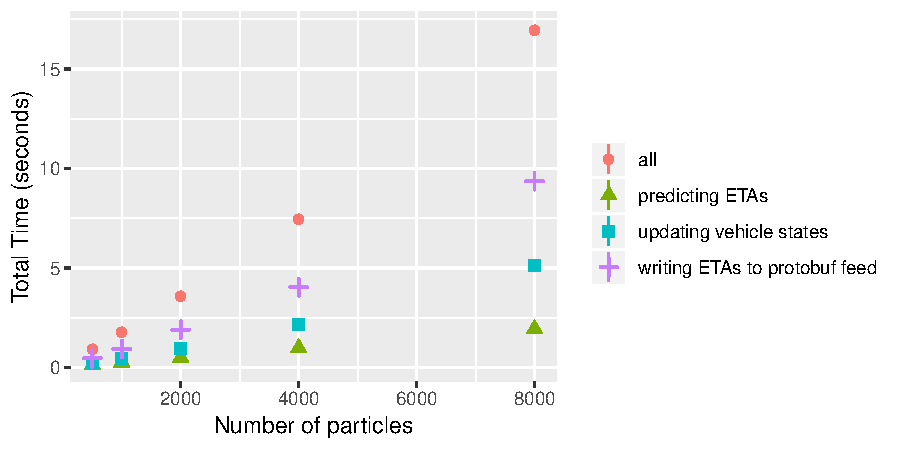
\includegraphics[width=0.7\textwidth]{figures/04_model_results_timing.pdf}
    \caption{The timings for various parts of the application, and overall. %
        The trend is slightly non-linear due to the complexity of the ETA generation step, %
        which requires sorting of the particle ETAs to obtain quantile estimates.}
    \label{fig:timings}
\end{figure}




\subsection{Model performance}
\label{sec:model_perf}


The model was evaluated using several statistics,
each calculated using a range of parameter values.
The first is effective sample size,
defined in (\ref{eq:neff}),
which is used to determined if resampling is required.
Another important statistic is the \emph{degeneration rate},
or the percent of iterations where the particle filter
is unable to find any plausible states given the observation,
and the vehicle is reinitialised.
Note, however, that the lower limit of this value 
is attributed to \emph{invalid trips},
however there is no simple way of filtering these trips.
The last statistic we compute is the variance of road segment travel times
over time.
For this example, we varied the number of particles $N$,
GPS error $\epsilon$, and system noise $\sigma^2$.


The one parameter we can determine from the data is GPS error, $\epsilon^2$,
by looking at the distance between observations and the shape.
Figure~\ref{fig:dist_to_route} shows the distribution of distance between the vehicle
observation and the \emph{nearest point on the path}.
Due to the way the observations are reported, 
many observations will be ``exactly'' on the route at a bus stop,
which explains the spike at just above zero~meters.

\begin{figure}[tb]
    \centering
    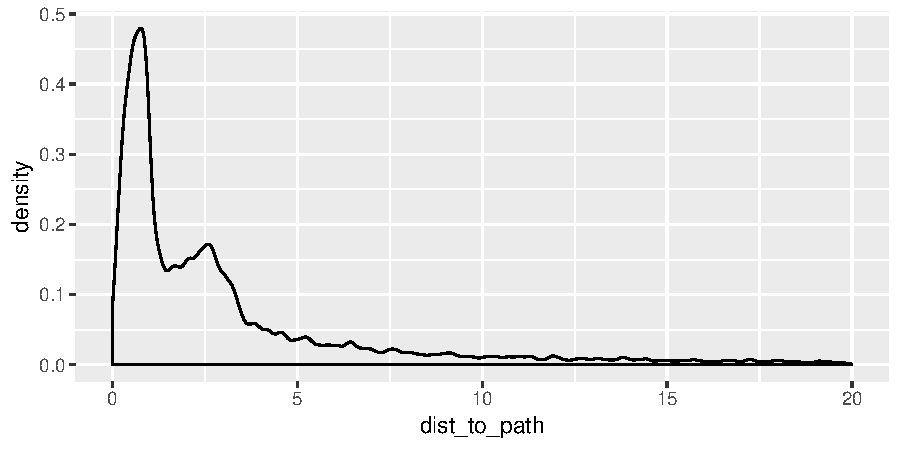
\includegraphics[width=0.7\textwidth]{figures/04_model_results_dist.pdf}
    \caption{The distance between the observation and the nearest point on the shape.}
    \label{fig:dist_to_route}
\end{figure}


For the effective sample size, 
increasing GPS error and system error both tend to
increase $N_\text{eff}$, as shown in Figure~\ref{fig:degen_rate}.
Increasing the GPS error distributes the weights more evenly,
while increasing system noise allows more particles to reach
the necessary speed,
so these are as expected.

\begin{figure}[tb]
    \centering
    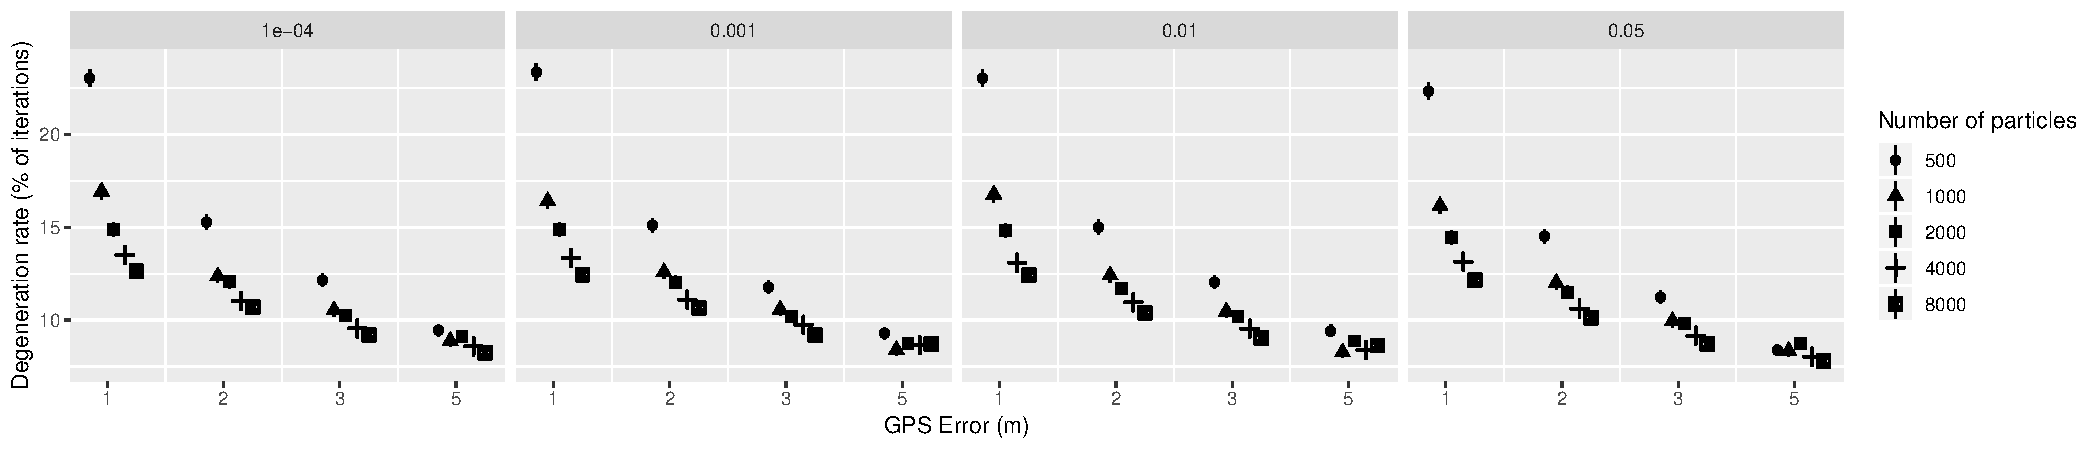
\includegraphics[width=0.9\textwidth]{figures/04_model_results_degen.pdf}
    \caption{The effective sample size and degeneration rate for a range of parameter 
        values. The columns are of increasing number of particles,
        and the rows are for increasing (downwards) GPS error.}
    \label{fig:degen_rate}
\end{figure}

The degeneration rate, 
shown on the $y$-axis of Figure~\ref{fig:degen_rate},
decreases as GPS error increases,
as anomolous observations where the bus is far from the route
are more likely.
It also decreases with the number of particles,
while system noise has no apparent effect.


Lastly is the variability of travel times and their uncertainties.
These are shown in Figure~\ref{fig:travel_times}.
System noise again shows no effect on the variability of travel time estimates,
however increasing GPS error tends to increase travel time variability.
This means that there is a trade-off between the models performance
and how well it estimates the main parameter of interest:
larger values of $\epsilon$ result in less degeneration and larger $N_\text{eff}$,
at the cost of more variable travel time estimates.


\begin{figure}[tb]
    \centering
    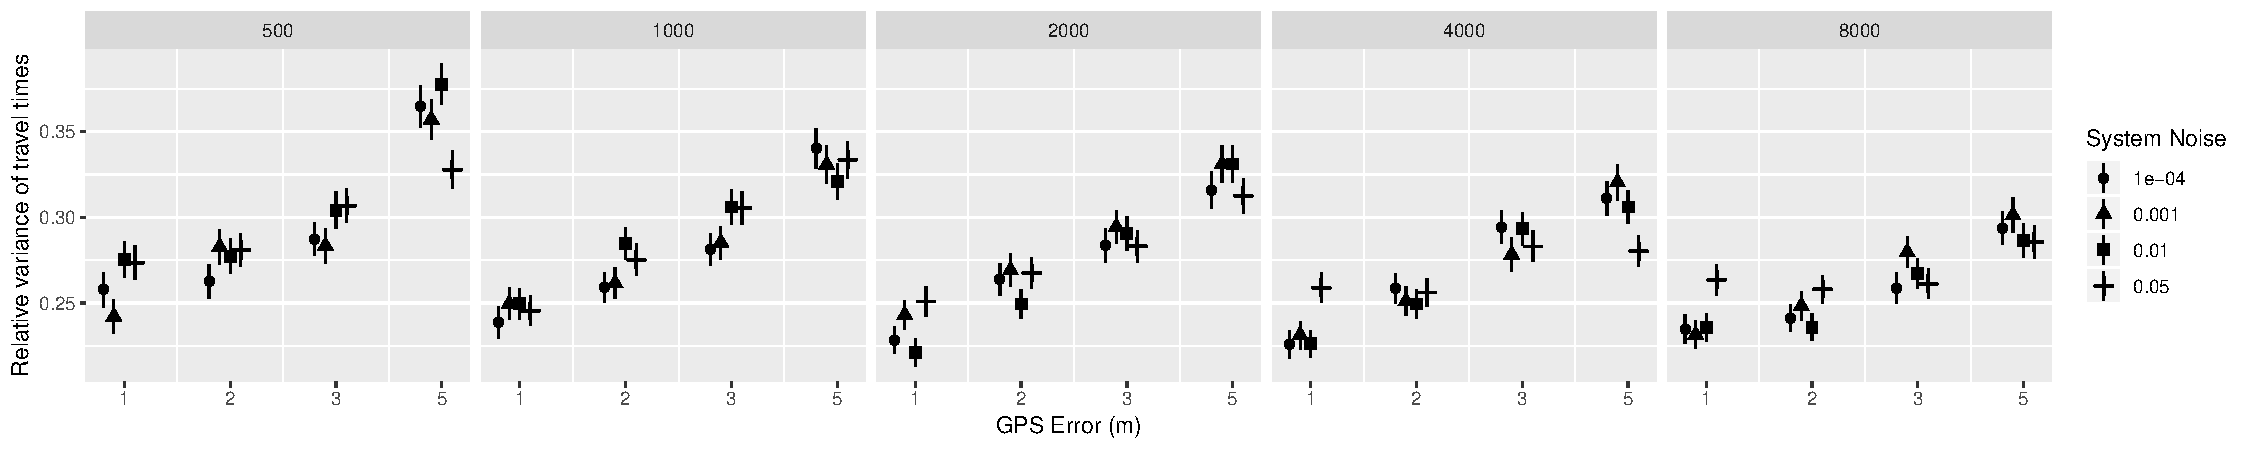
\includegraphics[width=0.9\textwidth]{figures/04_model_results_times.pdf}
    \caption{Travel times.}
    \label{fig:travel_times}
\end{figure}



\section{Preliminary Results}
\label{sec:results}

Currently only have timings (i.e., yes this is plausible).
- Function of number of particles/number of cores/number of buses.
- Network coverage? i.e., how many road segments actually get enough data
to generate useful numbers

- any problems?


\section{Discussion and Future Work}
\label{sec:discussion}

It all seems to work (hopefully I don't need to change this D:)

Next steps include
- generating useful priors for ``fall back'' (i.e., no data, future) prediction
- develop and implement a more complex network update model (correlations, etc)
- prediction estimates (point vs interval)

\bibliographystyle{anzsj}
\bibliography{../reflist.bib}

\end{document}
